\documentclass[border=3pt]{standalone}
% Preâmbulo compartilhado pelos diagramas TikZ da aula 7 (Filtros Não Paramétricos)
\usepackage[T1]{fontenc}
\usepackage[utf8]{inputenc}
\usepackage{lmodern}
\usepackage{amsmath}
\usepackage{xcolor}
\usepackage{tikz}
\usetikzlibrary{arrows.meta,angles,quotes,decorations.pathmorphing,calc,
                positioning,shapes.geometric,shapes.misc,backgrounds,fit,
                math}

% Paleta (mesma dos SVGs originais)
\definecolor{dblue}{HTML}{2A5B8C}
\definecolor{dorange}{HTML}{B3541E}
\definecolor{dgreen}{HTML}{4A7C59}
\definecolor{dred}{HTML}{9C4B4B}
\definecolor{dcream}{HTML}{F4F1EA}
\definecolor{dshade}{HTML}{DDD7C9}

% Função gaussiana (não normalizada por padrão de escala visual)
\pgfmathdeclarefunction{gauss}{3}{%
  \pgfmathparse{1/(#3*sqrt(2*pi))*exp(-((#1-#2)^2)/(2*#3^2))}%
}

% Estilos comuns (prefixo d... para não colidir com chaves internas do pgf)
\tikzset{
  >={Stealth[length=2mm]},
  dguide/.style={gray!55, dashed, line width=0.4pt},
  daxis/.style={gray!60, line width=0.7pt, ->},
  dbody/.style={fill=black!3, draw=black!80, line width=1pt},
  dacc/.style={draw=dblue, line width=1pt},
  dlbl/.style={black!55, font=\small},
  dsub/.style={black!45, font=\footnotesize},
  dstate/.style={circle, draw=black!80, fill=dcream, line width=1pt,
                 minimum size=17mm, font=\large, inner sep=1pt},
  dobs/.style={circle, draw=black!80, fill=dshade, line width=1pt,
               minimum size=14mm, font=\large, inner sep=1pt},
  dbox/.style={rounded corners=2pt, draw=black!80, fill=dcream, line width=1pt,
               align=center, inner sep=6pt},
  dop/.style={circle, draw=black!80, fill=white, line width=1pt,
              minimum size=6mm, inner sep=0pt, font=\small},
  dtrans/.style={->, dblue, line width=1pt},
  dmeas/.style={->, dorange, line width=1pt},
  dcurve/.style={line width=1pt, dblue},
  dcurveb/.style={line width=1.4pt, dorange},
}

\begin{document}
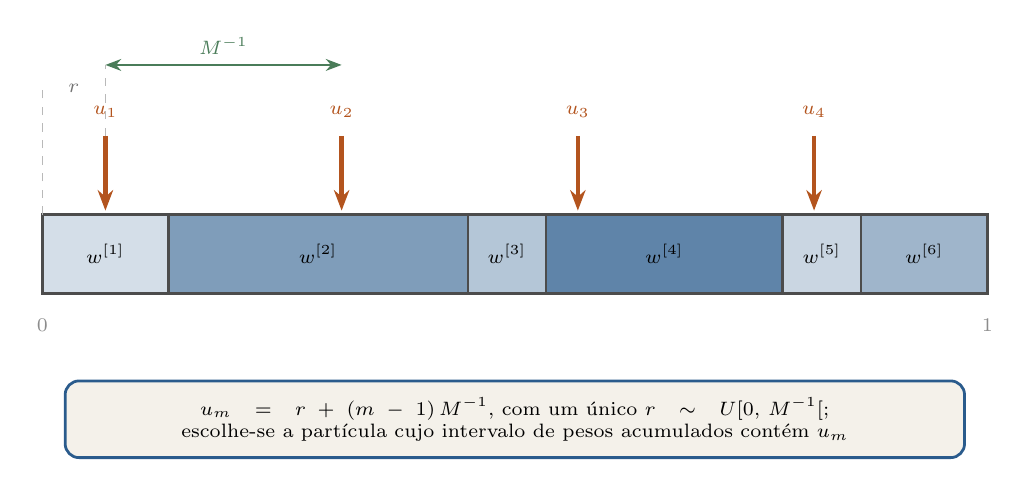
\begin{tikzpicture}[x=1cm,y=1cm]
  \draw[black!70, line width=1pt] (0,0) rectangle (12,1.0);
  \foreach \a/\b/\c/\i in {0/1.6/dblue!20/1, 1.6/5.4/dblue!60/2, 5.4/6.4/dblue!35/3, 6.4/9.4/dblue!75/4, 9.4/10.4/dblue!25/5, 10.4/12/dblue!45/6} {
    \fill[\c, draw=black!70, line width=0.8pt] (\a,0) rectangle (\b,1.0); \node[font=\scriptsize] at ({(\a+\b)/2},0.5) {$w^{[\i]}$}; }
  \foreach \u/\k in {0.8/1,3.8/2,6.8/3,9.8/4} {
    \draw[dorange, line width=1.6pt, -{Stealth[length=2.6mm]}] (\u,2.0) -- (\u,1.05); \node[dorange, font=\scriptsize] at (\u,2.3) {$u_\k$}; }
  \draw[<->, dgreen, line width=0.9pt] (0.8,2.9) -- (3.8,2.9) node[midway, above, font=\scriptsize] {$M^{-1}$};
  \draw[dguide] (0,1.0) -- (0,2.6); \draw[dguide] (0.8,2.0) -- (0.8,2.9); \node[dlbl, font=\scriptsize] at (0.4,2.6) {$r$};
  \node[dsub, font=\scriptsize] at (0,-0.4) {0}; \node[dsub, font=\scriptsize] at (12,-0.4) {1};
  \node[dbox, rounded corners=5pt, text width=11cm, font=\scriptsize, draw=dblue] at (6,-1.6) {$u_m = r + (m-1)\,M^{-1}$, com um único $r\sim U[0,\,M^{-1}[$; escolhe-se a partícula cujo intervalo de pesos acumulados contém $u_m$};
\end{tikzpicture}
\end{document}
